\section{Man, Woman, and Self}

In \textbf{Emmanuel Swedenborg}'s interpretation of Genesis, Eve appears as the “self” of Adam. The male principle is the Intelligence and the female principle symbolizes the Will. The Will is the “nucleus, the inmost heart of the human being.” The True Will, then, is man's true self …

How then does a man know his true Self, which is not something that can be observed directly, as one of the objects in the world? \textbf{E. F. Schumacher} outlined the four fields of knowledge\footnote{\url{https://www.gornahoor.net/?p=507}}. So, if I cannot adequately answer the question “Who am I”, then there is the question, “Who do you say I am?” A person usually deludes himself about who he is, whereas others easily see through his pretenses.

\begin{wrapfigure}{rt}{.3\textwidth}\centering
 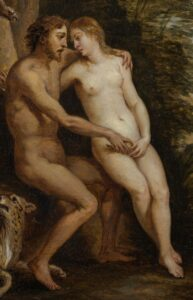
\includegraphics[scale=.7]{a20120908ManWomanandSelf-img001.jpg} 
 \caption{Adam And Eve In Paradise}
\end{wrapfigure}

If Swedenborg is providing the esoteric interpretation, the exoteric understanding is not precluded; to the contrary, it is necessary. For Adam, the Self is dead, represented by the rib since the bones are the last to decay. That rib is vivified by Eve, who appears therefore as the \emph{exteriorization} of his own Self. She is almost his identical twin, genetically the same apart from her having two X chromosomes, his “reciprocal”. Hence, she is the perfect woman for him. In knowing Eve, Adam is knowing himself.

Every woman desires a man who “gets” her, that is, someone who understands her in a deep way. The converse is not identical. A woman, too, wants to know her man, but not always just in his actuality, but also in his potentiality. This often comes across as a desire to change him, leading to a degree of conflict. If this conflict subsides, it indicates she has decided to “settle”, as they put it. On the other hand, it may impel the man to exceed himself. In \textit{Gnosis}\footnote{\url{https://www.gornahoor.net/library/mouravieff3.pdf}}, \textbf{Boris Mouravieff} provides, as examples, \textbf{Wagner} and \textbf{Goethe} who achieved great moments of creativity, inspired by infatuations with younger women.

Sometimes, even among the Medievalists, a woman is represented as an imperfect man. However, that is putting her on the wrong scale, as there do exist imperfect men on the scale whose peak is the Absolute Male. A woman can only be represented on the corresponding scale with the Absolute Female at its peak.

This is a difficult teaching. If the woman is the perfect helpmeet for a man, why is it not always experienced that way? In a relationship, a man is, in some deep way, confronting his own self. To the degree that he lacks self-awareness, the less he sees that. Mouravieff writes:

\begin{quotex}
just as one particular woman produces a different effect of carnal attraction on different types of men, so, on the psychic plane, the creative spirit of a man produces a different psycho-sexual attraction on different women. 

\end{quotex}
The complexities of attraction must be understood on the three levels: carnal, psychic, and spiritual. So called “success” at the carnal level can be mastered if desired. An intelligent man can make changes to himself as he learns to master himself. However, although that is celebrated in the modern world, it is not likely the best use of one's inner resources. Often, a man will entangle himself in harmful karmic relationships that become difficult to extract himself from.

The lower a man is on the scale of the Absolute Male, there is less and less differentiation. Hence, the woman attracted by such a man is likely to be very much like him. At the lowest levels, the lack of differentiation may even appear as an attraction to the same gender. There is little challenge in this case and hence less possibility of achieving self-knowledge.

The higher on the scale, then, the woman will also be correspondingly higher, thereby deviating more and more from each other. That is, ultimately the Absolute Man will attract the Absolute Female, and their respective qualities will be quite different from each other. This hardly means that things go so smoothly, as the higher stages of self-realization get more difficult. In one incident, \textbf{Dante} passed Beatrice and two of her friends on a street in Florence. When she snubbed him, he was so upset he hid in an alley and cried for hours.

Yet Beatrice was the one who prayed for Dante on his journey to Paradise, and became his ultimate guide to the Supreme Identity. Scholars today still debate the identity of Beatrice. But Gornahoor readers now know exactly who she is.


\hfill

For further reading, see Swedenborg and Esoteric Islam by Henry Corbin.



\flrightit{Posted on 2012-09-08 by Cologero }

\begin{center}* * *\end{center}

\begin{footnotesize}\begin{sffamily}



\texttt{O on 2016-12-09 at 20:45 said: }

If the Absolute Man is the same as the sexually differentiated Adam prior to the fall from the centre of the human state, what happens if the spiritual reintegration goes deeper still, becoming the Primordial Androgynous Man? Can we still speak of the Absolute Man if it doesn't have Absolute Woman as its opposite pole, precisely because both poles are reintegrated into the principle preceding them? What is the reaction of the Absolute Woman to a being having realised that state, integrated his opposite and hence become completely free of desire?


\hfill

\texttt{Cologero on 2016-12-11 at 10:45 said: }

@O, I don't think we want to understand “Absolute Man” in such biological terms. Rather, it is the union of the Intelligence and the Will, the head and the heart. Such as we are, the Will and the Intellect are not united, they are usually at war with each other. It is as though we have multiple selves. In Hermetic terms, this union is the alchemical marriage: the Holy Spirit (intelligence) is reflected in the soul (will) giving birth to the Christ, or Logos, as the true self.


\hfill

\texttt{O on 2016-12-11 at 20:29 said: }

That is succinctly put, Cologero, and I agree. But the article differentiates between `Absolute Man' and `Absolute Woman'. which of course is well known from Evola. That is a `sexual' distinction on an archetypal level, but not necessarily a biological phenomenon as known in our existential state. (I think it was C.S. Lewis who wrote somewhere that `gender' differentiation in beings is manifested in modes more essential than biological sex.) What you now explained seems to be different from the notion of an Absolute Man having as his opposite an externally manifested/embodied Absolute Woman, which would be a dual and complementary relation.


\hfill

\texttt{Cologero on 2016-12-11 at 21:33 said: }

@O, rather than repeat myself, perhaps you could comment on this: Absolute Man, Absolute Woman.

Aren't Yin and Yang the ultimate distinction? I believe that the Tao, then, is the union. The Chinese translate the word “Logos” by “Tao”.


\hfill

\texttt{Max on 2019-09-09 at 14:12 said: }

Swedenborg also treats the subject of Polar Beings in his book “Conjugal Love”. So far, I have only had time to eye through it rather briefly, and there seems to be both agreements and some differences when compared to Mouravieff's teaching. From memory, Swedenborg maintains that the prospective polar beings will increasingly polarize according to their efforts, and gradually adapt to one another. There is a potential polarity which is only effectively realised through the sacrament of marriage and conjugal love. In other words, the perfectly polar couple is most likely not found in some sort of “state of nature”. First of all they must crucially be able to recognize one another, which is heavily stressed by Mouraieff.


\end{sffamily}\end{footnotesize}
